\documentclass[10pt,landscape,a4paper]{article}
\usepackage{multicol}
\usepackage[landscape]{geometry}
\usepackage{hyperref}
\usepackage[utf8]{inputenc}
\usepackage{minted}
\usepackage{graphicx}
\usepackage[binary-units]{siunitx}
\usepackage[usenames]{xcolor}

\geometry{top=1cm,left=1.5cm,right=1cm,bottom=1cm}

% Turn off header and footer
\pagestyle{empty}
 
% Redefine section commands to use less space
\makeatletter
\renewcommand{\section}{\@startsection{section}{1}{0mm}%
                                {-1ex plus -.5ex minus -.2ex}%
                                {0.5ex plus .2ex}%x
                                {\normalfont\large\bfseries}}
\renewcommand{\subsection}{\@startsection{subsection}{2}{0mm}%
                                {-1explus -.5ex minus -.2ex}%
                                {0.5ex plus .2ex}%
                                {\normalfont\small\bfseries}}
\renewcommand{\subsubsection}{\@startsection{subsubsection}{3}{0mm}%
                                {-1ex plus -.5ex minus -.2ex}%
                                {1ex plus .2ex}%
                                {\normalfont\footnotesize\bfseries}}
\renewcommand{\paragraph}{\@startsection{paragraph}{3}{\z@}%
                                {-1ex plus -.5ex minus -.2ex}%
                                {-.5em}%
                                {\normalfont\scriptsize\bfseries}}
\makeatother

% Don't print section numbers
\setcounter{secnumdepth}{0}

\setlength{\parindent}{0pt}
\setlength{\parskip}{0pt plus 0.5ex}

% Compact lists
\usepackage{enumitem}
\setlist{nosep}

% -----------------------------------------------------------------------

\begin{document}

\footnotesize
\begin{multicols*}{3}

% multicol parameters
% These lengths are set only within the two main columns
%\setlength{\columnseprule}{0.25pt}
\setlength{\premulticols}{1pt}
\setlength{\postmulticols}{1pt}
\setlength{\multicolsep}{1pt}
\setlength{\columnsep}{2pt}

\section{Speicher / Caches}

\begin{description}
  \item[RAM-Aufbau] In Zeilen und Spalten, es wird immer eine Zeile gelesen
    $\rightarrow$ bursty reads sind schneller
  \item[SRAM] Statisch, mehr Bauteile $\rightarrow$ teurer
  \item[DRAM] Dynamisch, weniger Bauteile (R/C), braucht alle 64ms refresh
  \item[Speicherhierarchie] Volatile (register/cache/RAM), Non-Volatile (SSD,
    HDD, $\ldots$). $\uparrow$: CPU-Distanz/Kapazität/Fehlerraten; $\downarrow$:
    Geschwindigkeit, Preis pro Byte
  \item[Lokalität (Zeit)] \verb|s += a[i]| in einem loop: Wenn \verb|s| jetzt
    gebraucht wird, vermutlich auch demnächst
  \item[Lokalität (Raum)] lokale Variablen sind in der Nähe im RAM: Wenn
    \verb|a| gebraucht wird, dann vermutlich auch \verb|a + 1|, $\ldots$
\end{description}


\subsection{Timing}

\begin{itemize}
\item $T_c$: Zugriffszeit auf Cache
\item $T_M$: Zugriffszeit auf RAM ($T_M >> T_C$)
\item $p_c$: Wahrscheinlichkeit von cache hit - Wegen Lokalität oft $90\% - 100\%$
\item Durchschnittliche Zugriffszeit: $E(T) = p_cT_c + (1-p_c)T_m$
\end{itemize}

\subsection{Typen}

\subsubsection{Fully associative cache}

\verb|tag(A) = A|; cache speichert volle Adresse. Müsste quasi eine Hashmap in
Hardware implementieren, oder iterativ O(n). Daher oft $< \SI{4}{\kilo\byte}$.

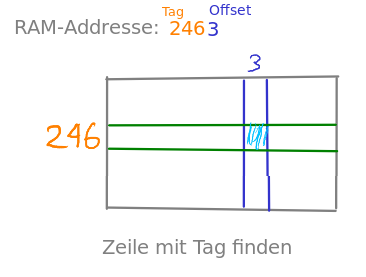
\includegraphics[width=0.5\linewidth]{cache_fully.png}

\subsubsection{Direct mapped}

\verb|tag(A) = A[m..n-1]|; wir maskieren die Adresse. Einfach und schnell, aber
viele Kollisionen - wir brauchen also mehr Kapazität.

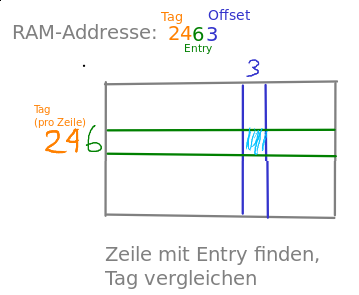
\includegraphics[width=0.5\linewidth]{cache_direct.png}

\subsubsection{$k$-way set associative}

Wir haben $k$ direct mapped caches, d.h. wir können pro way/set-Paar ein Entry haben.

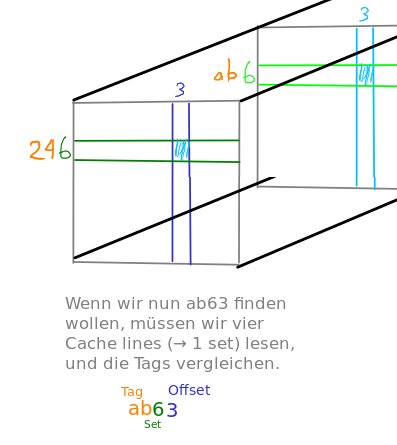
\includegraphics[width=0.5\linewidth]{cache_kway.png}


\paragraph{Speicherbedarf (k-way)}

\begin{itemize}
  \item z.B. \SI{32}{\kilo\byte} cache, 4-way; $l = \SI{64}{\byte}$ (Cachezeilenlänge)
  \item Cachezeilen $z = \SI{32}{\kilo\byte} / \SI{64}{\byte} = 2^{15} / 2^6 =
    2^9 = 512$ \\ ($\rightarrow$ pro way: $z' = 128$)
  \item Offset (Spalte) braucht $log_2{(l)}$ ($\rightarrow$ 6)
  \item Set (Zeile) braucht $log_2(z')$ ($\rightarrow$ 7)
  \item Tag braucht den Rest, bei Adressbreite von 64bit z.B. \\ $64 - 6 - 7 = 51$
\end{itemize}

\subsection{Zugriff}

\begin{description}
  \item[R: Look-Aside] Zugriff geht gleichzeitig auf Bus und Cache. Entweder
    legt der Cache den Wert auf den Bus (hit), oder der Cache liest den Bus
    (miss). Einfacher und günstiger.
  \item[R: Look-Through] Zugriff geht direkt auf den Cache, Cache kommuniziert mit
    Bus (falls miss). Weniger Bus traffic.
  \item[W: Write-Through] Synchron, CPU schreibt Daten zum Cache/RAM und wartet auf
    beide.
  \item[W: Write-Back] Asynchron, CPU schreibt Daten zum Cache, Cache schreibt die
    Daten ins RAM. Problem: Cache-Koheränz bei Multiprozessor-Systemen.
\end{description}


\section{Dynamischer Speicher}

\begin{description}
  \item[Stack/Heap] Stack kann dynamisch Speicher allozieren, hat aber eine
    beschränkte Grösse.
  \item[double free] Grösse des Blockes wird für \verb|free| direkt vor dem
    Block gespeichert. Mit double-free wird aber beliebiger Wert als Grösse
    angenommen.
  \item[memory leak] Speicher wird nie freigegeben (obwohl es keinen Pointer
    mehr darauf gibt) - problem bei expliziter Freigabe.
  \item[interne Fragmentierung] Interne Block-Grösse ist grösser als
    angeforderter Bereich $\rightarrow$ waste
  \item[externe Fragmentierung] Programm fordert unterschiedlich grosse
    Speicherbereiche an, gibt gewisse wieder frei, es entstehen Lücken.
\end{description}


\subsection{Implementierung}

\subsubsection{Fixe Blockgrösse}

Speicher wird in fixe Blöcke unterteilt. Variable Zuordnungsgrösse: Spezialfall
mit Blockgrösse 1. Blockgrösse ist ein Tradeoff zwischen wenig Fragmentierung
(kleine Blöcke) und bessere Performance bzw. weniger Metadaten (grosse Blöcke).

\subsubsection{Object pools}

Ein Block (bzw. Page) wird in kleinere Blöcke (für je 1 bestimmtes Objekt) mit
fixer Grösse aufgeteilt. Wenig/keine Verschwendung; Rekombination entfällt.
Freiliste mit freien Objekten.

\subsubsection{Buddy-System}

Ähnlich wie beim \emph{quick fit}-Algorithmus gibt es verschiedene Blockgrössen,
jeweils $2^k$. Blöcke werden in Zweiergruppen geteilt:

\begin{verbatim}
[               ] (32, n=6) 00000 (requested: 3B)
[       ][ 16 f ] (n=5)     00000 / 10000
[   ][8f][      ] (n=4)     00000, 01000  / 10000, 11000
[][][   ][      ] (n=3)     00000, 00100  / 01000, 01100 / …
4!4f  (4 used, 4 free)      ^- buddies -^ (nur bit n anders)
\end{verbatim}

Reservation: Suche passenden Block (angeforderte Grösse auf $2^k$ aufgerundet).
Falls nicht vorhanden: Finde nächstgrösseren Block und zerteile ihn.

Freigabe: Kombiniere (nur) \emph{mit Buddy-Block} falls möglich (rekursiv).

\subsection{Metadaten}

\subsubsection{Dezentral}

Metadaten direkt vor/nach Speicherblöcken. Schnelle Rekombination, aber kein
Schutz vor z.B. array overflows (ausser mit magic numbers).

\subsubsection{Zentral}

Eigene Datenstruktur für Metadaten. Entweder fixe Grösse oder mehr Komplexität,
aber Schutz vor Überläufen.

\begin{description}
  \item[Bitliste] 1 bit pro Speicherblock, used/free. Suche nach
    Speicherbereich: Suchen nach genug langer 0-Kette (kann lange dauern).
  \item[Linked list] Liste mit \verb|(is_free, *start, size)|
    Elementen, sortiert nach Adresse. Einfaches Suchen; einfaches Zusammenführen
    von freien Nachbarn nach \verb|free|.
\end{description}

\subsection{Suchalgorithmen}

\begin{description}
  \item[First Fit] Nimmt erste passende Lücke - Ansammlung von vielen
    kleinen Lücken am Anfang.
  \item[Next Fit] Nimmt erste passende Lücke nach zuletzt reserviertem Bereich.
    Kleine Lücken überall, daher schlechter als FF.
  \item[Best Fit] Durchsucht ganze Liste nach bester Lücke. Sehr langsam, mehr
    Verschwendung da verbleibende Lücken zu klein sind, um genutzt zu werden.
  \item[Worst Fit] Wie BF, sucht aber nach grösster Lücke. Langsam, keine guten Ergebnisse.
  \item[Quick Fit] Verschiedene Grössenklassen (z.B. $1..n$ oder $2^n$) mit
    eigenen linked lists. Allozierung wählt nächstes freies Element der
    passenden Klasse. Sehr schnell, aber Rekombination ist aufwändig (Nachbarn
    sind schwer zu finden).
\end{description}

\section{Virtueller Speicher}

\begin{description}
  \item[Realer Speicher] Programm kriegt echte Addressen, ggf. zur Laufzeit
    umgeschrieben für Relokation. Speicherschutz möglich (Code-Register das nur
    vom OS geschrieben werden kann mit Code pro Prozess, oder Limit-Register für
    relative Addressen).
  \item[Translation Lookaside Buffer] Speichert häufig genutzte page mappings (Lokalität)
  \item[Memory mapped file] Echte Datei statt swap-file via RAM
\end{description}

\subsubsection{Grundlagen}

MMU RAM und CPU/Prozess. Das OS konfiguriert
die MMU, der Prozess kennt nur virtuellen Addressen von der MMU.

Bei ungültigem Zugriff signalisiert die MMU einen Fault Interrupt zum OS.
Bei Swapping lädt das OS die Page von Sekundärspeicher ins RAM und
passt mapping table an (MMU kennt nur RAM!).

Speicher basiert auf \emph{pages}, die meist \SI{4}{\kilo\byte} gross sind.
Hauptspeicher wird in \emph{page frames}
unterteilt. Bei einer Addresse wie \verb|0xAB 78 9C CC| ist dann \verb|0xAB789|
die page frame number, und \verb|CCC| (12 LSB) der Offset.

\subsection{Page Tables}

Die MMU muss wissen, ob eine page gültig ist, und in welchem page frame sie ist.
Das OS muss wissen, wo die page ist (Haupt-/Sekundärspeicher), ob sie verwendet
wird, und ob sie seit dem letzten Einlagern verwendet wurde.

\subsubsection{Single level}

Array mit \verb|(page_num, status_bits)| für jede page, mit page number als
index.

Wenn Prozess auf \verb|0x8765431| zugreift, ermittelt die MMU die page number
\verb|0x8765|, schaut in der page table da nach, findet \verb|0xABCD0| $\rightarrow$
Addresse ist also \verb|0xABCD0321|. Wird sehr schnell gross, Beispiel:

\begin{itemize}
  \item \SI{4}{\kilo\byte} page size ($2^{12} \si{\byte}$); 32-bit Addressen \\
    $\rightarrow log_2({\SI{4}{\kilo\byte}}) = 12$ bits Offset
  \item \SI{4}{\giga\byte} RAM ($2^{32} \si{\byte}) / \SI{4}{\kilo\byte} =
    2^{20}$ (1M) page frames \\ $\rightarrow \SI{20}{\bit}$ page nr
  \item \SI{4}{\giga\byte} virtueller Speicher $\rightarrow 1M$ Einträge
  \item \SI{32}{\bit} pro Eintrag (page nr + statusbits)
  \item Page table ist \SI{4}{\mega\byte} pro Prozess!
\end{itemize}

\subsubsection{Two level}

Page number wird in \emph{directory index} und \emph{page table index}
aufgeteilt. Es gibt mehrere page tables. Das page directory (für jede page table)
sowie die page table (für jede page) haben ein used-bit.

\begin{verbatim}
page_table = page_directory[directory_index]
page = page_table[page_table_index]
\end{verbatim}

Beispiel:

\begin{itemize}
  \item Prozess will \verb|0x87654321|
  \item Directory index: \verb|0x21D|  % FIXME warum?
  \item Page number: \verb|0x254|
  \item MMU schaut bei Index \verb|0x21D| nach, kriegt pointer auf secondary
    level page table (\verb|0x2000|)
  \item MMU schaut in SLPT an Index \verb|0x254|, kriegt frame number \verb|0xABCD0|
  \item Reale Addresse: \verb|0xABCD0321|
\end{itemize}

Mit $2^{10}$ Einträgen pro Page haben wir so $2^{20}$ Pages pro Prozess!

\subsection{IPC}

\begin{description}
\item[Shared memory] Prozesse teilen sich Speicher. Verschiedene Page Frames (in den
zwei Prozessen) zeigen auf gleiche Page.
\item[Message passing] OS kopiert daten zwischen zwei unabhängigen pages/frames. Mehr
Isolation, aber Overhead.
\end{description}

\subsection{Page tables auf x86}

Jede Page hat ein \verb|P| (present) bit. Mit \verb|P = 1|: MMU-spezifisches
Layout mit Page Frame und status bits (u.a. ``Accessed'' für jeden Zugriff,
``Dirty'' bei Schreibzugriff). Mit \verb|P = 0|: MMU wirft interrupt, OS kann
beliebige Infos (Ort im Sekundärspeicher) in der table speichern. OS wirft
segfault bei ungültigen Infos.

\subsection{Paging-Strategien}

\subsubsection{Ladestrategien}

Welche Page wird wann geladen? Beeinflusst Häufigkeit von Page-Faults.

\begin{description}
\item[Demand Paging] Paging werden auf Anfrage bei Interrupt geladen. Minimaler
  Aufwand, aber lange Wartezeiten für den Prozess bei jedem page fault.
\item[Prepaging] System versucht heuristisch zu ermitteln, welche Pages
  gebraucht werden.
\item[Demand Paging mit Prepaging] Lokalität: Wird eine Page gebraucht, werden
  vermutlich auch Nachbarn gebraucht und spekulativ mitgeladen.
\end{description}

\subsubsection{Entladestrategien}

Wann werden im RAM modifizierte Pages zurück geschrieben? Beeinflusst
Verzögerung bei Page Fault.

\begin{description}
\item[Demand cleaning] Page wird zurück geschrieben wenn Frame wiederverwendet
  werden soll. Minimaler Aufwand, erhöhte Wartezeit für Prozess der neue Page
  braucht
\item[Precleaning] Page wird frühzeitig in Sekundärspeicher geschrieben.
  Reduzierte Wartezeit, aber wenn Page nach Schreibvorgang nochmals verändert
  wird schlecht.
\item[Page Buffering] OS hat Liste von un-/modifizierten pages. Unmodifizierte
  werden zuerst ersetzt, modifizierte werden als batch geschrieben und in die
  andere Liste verschoben. Prozess kriegt schnell neue Page.
\end{description}

\subsubsection{Verdrängungsstrategien}

Welche Page wird aus dem Hauptspeicher entfernt, wenn Speicher knapp ist?

MMU setzt R-bit (referenced/accessed) bei jedem Lese-/Schreibzugriff, OS löscht
es z.B. periodisch. MMU setzt M-bit (modified/dirty) bei Schreibzugriff, OS
löscht es nachdem page zurückgeschrieben wurde. Pages mit M=0 werden bevorzugt
ersetzt (zurückschreiben nicht nötig).

\begin{description}
  \item[optimal] Ersetze Page, die am spätestens in der Zukunft gebraucht werden
    wird. Unrealistisch in der Praxis (ausser bei genau bekanntem Verhalten), aber
    Referenz als Grenze des Machbaren.
  \item[FIFO] Braucht keine Status bits, ersetze älteste Seite nach Ladezeitpunkt.
    Alte, häufig benutzte Seiten werden immer wieder entfernt und geladen; mehr
    RAM kann zu mehr faults führen (\emph{Beladys Anomalie})
  \item[Second chance] Wie FIFO, aber R-bit der letzten Page wird geprüft. R=0:
    Wurde nicht benutzt $\rightarrow$ weg; R=1: \verb|R := 0|, page an das Ende
    der LL $\Rightarrow$ entfernt älteste nicht verwendete Page
  \item[Clock] Effizientere Implementierung mit circular linked list und next-pointer.
  \item[LRU] MMU notiert Timestamp bei jedem Zugriff. Sehr gut, aber grosser
    HW-Aufwand; grössere Page-Einträge.
  \item[NFU] (not frequently used) Pro Page ein counter, periodischer Interrupt
    inkrementiert counter, ersetze Page mit niedrigstem counter. Alte Pages
    (früher oft verwendet) haben aber einen hohen counter selbst wenn sie nicht
    mehr genutzt werden.
  \item[NFU mit aging] counter ist Verlauf: \verb|cnt = (cnt >> 1) + (R << n)|
  \item[Working Set] Behalte Pages im ``Arbeitsbereich'' mit Intervall $T$. Jede
    Page hat ein timestamp $t$. Bei Fault interrupt werden alle pages gescannt;
    wenn \verb|R = 1| wird $t$ aktualisiert, wenn \verb|R = 0| wird entfernt
    falls $\Delta{}t < T$. Fallback: älteste page.
  \item[WSClock] Circular linked lists mit zusammenhängenden Pages
\end{description}

\section{I/O}

\begin{description}
\item[Memory mapped] Gerät hat Adressbereich der wie Speicher benutzt wird.
  Diese Adressen können aber nicht für RAM benutzt werden. Einfach
\item[Port mapped] Eigener IO Bus und Addressraum. CPU braucht zusätzliche Logik
  (und Instruktionen), System braucht zusätzlichen Bus.
  \begin{description}
    \item[via Speicherbus] RAM-Bus hat zusätzliches selector bit, CPU
      hat I/O-Instruktionen. Wie Port mapped, aber Systemdesign ist einfacher.
  \end{description}
\item[Polling] Normalerweise schlecht, aber (bei schnelleren Geräten) bessere
  (und deterministischere) Performance.
\item[Interrupt Controller] Hängt an allen Devices die einen Interrupt senden
  wollen. Signalisiert Interrupt der CPU und gibt Interrupt-Nummer an.
\item[DMA] Eigener Controller - CPU programmiert DMA und gibt Bus frei, DMA
  lässt das Gerät direkt die Daten auf den Bus kopieren und setzt Interrupt.
  \begin{description}
  \item[Einzeltransfer] DMA nutzt Bus nur für einen Transfer (periodisch wenige
    Daten)
  \item[Blocktransfer] DMA belegt Bus länger, wenn Gerät viele Daten liefern
    kann (z.B. HDD, NIC)
  \end{description}
\item[Treiberarchitektur] \strut
  \begin{description}
    \item[Ohne] Programme kommunizieren direkt mit der Hardware.
      Sicherheit/Stabilität ist ein Problem, und Programme sind komplexer.
      Nur ein Prozess kann auf die Hardware zugreifen.
    \item[Mit] OS stellt API für die Hardware bereit; OS hat einen Treiber
      (generisch, vom Hersteller, …). Treiber laufen meist im Kernel-Mode.
    \item[Microkernel] Treiber sind Prozesse im User-Mode, generischer
      Interrupt-Handler der Treiber-Prozesse anstösst. Stabiler aber langsamer.
  \end{description}
\end{description}

\pagebreak

\section{GUIs}

\begin{description}
  \item[Baumstruktur] Bildschirm ist das root window, Fenster haben Unterfenster (widgets).
  \item[Fenster] Rechteckiger Bereich des Bildschirms
\end{description}

\subsubsection{Windows}

\begin{description}
  \item[Handle] Pointer auf ein Objekt (repräsentiert OS-Ressource), opaque
  \item[MSG struct] Enthält Fenster-Handle, event type, params,
    Zeitstempel, Hotspot (Pixel im Mauscursor). Für alle Messages gleich gross.
  \item[Keyboard messages] \verb|TranslateMessage()| macht \verb|WM_CHAR|
    message mit char-Code aus \verb|WM_KEYDOWN| mit scancode.
  \item[Window procedure] Callback fürs OS, welches Messages akzeptiert. Wird
    via window class mit Message-Typ assoziiert. \verb|DefWindowProc()| ist die
    default window procedure, muss für alle Messages die von \verb|WndProc|
    nicht bearbeitet wurden aufgerufen werden.
  \item[Window class] Definiert window procedure, style, Menü, etc. für ein
    Fenster. Es gibt vordefinierte Klassen, oder es können benutzerdefinierte
    via \verb|RegisterClass| registriert werden. Wird über Name (String)
referenziert.
  \item[Message Queue] FIFO von Messages. Einige Typen
    (\verb|WM_PAINT|/\verb|_QUIT|/\verb|_TIMER|) werden erst am Schluss
    abgearbeitet, \verb|WM_PAINT| wird zusammengefasst. Auch Dinge wie ``Text
    setzen'' passieren via messages (an eigenes Window). Nur GUI-threads haben Queue.
   \item[PostMessage()] fügt Message am Ende ein (non-blocking für
     caller). Gibt \verb|bool| zurück (queuing OK). Mit \verb|NULL| als handle
     in eigene Queue.
   \item[SendMessage()] ruft direkt window procedure auf (blocking für
     caller). Gibt \verb|LRESULT| zurück, kann bei mehreren Threads zu Deadlocks führen.
   \item[GetMessage()] Wartet blockierend, gibt 0 bei \verb|WM_QUIT| zurück. Hat
     Filter für Window und Type (min/max).
   \item[Ressourcen] Windows hat einen resourcen-Compiler der einige
     C-Präprozessor-Direktivne kann. Darin sind ressourcen-Definitionen, die
     dann zu \verb|.res| kompiliert werden, was der Linker versteht..
   \item[Device-Context] Abstraktion von Gerät (z.B. Bildschirm, Fenster,
     Drucker), das z.B. auch Font und ``Framebuffer'' für das Gerät enthält.
     Kann geklont werden (z.B. um vorzuzeichnen).
\end{description}


\begin{minted}{c}
int WinMain(...) {  
  RegisterClass(...);
  CreateWindow(...); 
  while(GetMessage(...)) { 
    TranslateMessage(...); 
    DispatchMessage(...);
  }
} 

LRESULT WndProc(....) { ... } 
\end{minted}

\columnbreak

\subsection{Unicode}

\begin{description}
  \item[UTF-32] Ein Codepoint als 4 byte direkt (big/little endian)
  \item[UTF-8] Superset von ASCII. Keine Endianness.
  \item[UTF-16] LE/BE, 2 byte.
  \item[Windows] Intern UTF-16, diverse API die doppelt als \verb|A| und
    \verb|W| Variante existiert.
  \item[Code Unit] 8/16/32-bit unit in UTF-8/16/32
\end{description}

\subsection{X}

\begin{description}
  \item[Puffer] Puffer existiert auf Client und auf Serverseite (möglichst wenig Traffic!)
  \item[Window classes] InputOutput und InputOnly.
  \item[Ressourcen] Infos mit IDs, z.B. Pixmap/font/...
  \item[Grafikfunktionen] Rastergrafik mit Farbtabellen, primitives, Font.
    Brauchen graphics context für Liniendike, Farben, etc.
  \item[Events] Typ \verb|XEvent|, union über alle Event-Typen (also so gross
    wie der grösste Typ). Erster Member ist ein \verb|type| int, Code wählt
    damit den passenden Union-Member.
  \item[Fehlerbehandlung] Rückgabewerte, \verb|XSetErrorHandler()| (Protokoll),
    \verb|XSetIOErrorHandler| (fatal)
  \item[Display] Rechner mit Tastatur/Pointing device/screen
\end{description}

\begin{minted}{c}
while (true) {
  XNextEvent(display, &event);
  switch (event.type) 
  {
  case Expose:
    ...
    break;
  ...
  }
}
\end{minted}

\section{Dateisysteme}

\begin{description}
  \item[File-Deskriptor] Index in die Tabelle der geöffneten Dateien (pro Prozess)
  \item[Volume] Datenträger oder Partition
  \item[Hardlink] Mehrere Pfade oder Inode-links für dieselbe Datei
\end{description}

\subsection{FAT32}

\begin{description}
  \item[Bootsektor] Enthält Sektorengrösse, Anzahl Sektoren pro Cluster, Anzahl
    FATs und Grösse, Volumegrösse, Label, etc.
  \item[Cluster] Fässt Sektoren von Dateien zusammen.
  \item[FAT] Enthält Clusterketten-Eintrag pro Cluster (erster Cluster einer Datei). Der
    Eintrag zu diesem Cluster hat dann die Addresse des nächsten Clusters (oder
    Ende-Zeichen). Es gibt ein Backup.
  \item[Verzeichnis] Eintrag der auf weitere Directory/File Entries zeigt.
  \item[Eintrag] 8.3 filename, Clusternummer, Flags, Size, Timestamps
\end{description}

\columnbreak

\subsection{NTFS}

\begin{description}
  \item[Konzept] ``Alles ist eine Datei'' (auch Metadaten)
  \item[Bootsektor] Enthält nur Dinge wie Sektorengrösse, Sektoren pro Cluster,
    Cluster der MFT, etc.
  \item[MFT] Beschreibt Dateien, selber auch eine Datei. Mehrere Kopien.
  \item[Records] Liste von Attributen (aka Streams)+ Endmarker.
  \item[Attribute] Die meisten Attribute sind optional. Entweder Name oder Typ
    muss sich unterscheiden. Entweder resident (komplett im record, z.B.
    Dateiname) oder non-resident (wird ausserhalb der MFT fortgesetzt).
    Selbst \verb|$DATA| kann für kleine Dateien resident sein.
  \item[Runlist] Sequenz von Runs. Ein Run sind mehrere aufeinanderfolgende
    Cluster.
  \item[Komprimierung] NTFS hat sparse files, Run ohne Adresse in Runlist. Kann
    aber LZ77 wenn damit Cluster eingespart werden, setzt als placeholder dann
    Sparse-Run ein.
\end{description}

\subsection{Ext}

\begin{description}
  \item[Block] Mehrere Sektoren, entspricht Clustern. Es ist aber das ganze Volume
    aufgeteilt in Blöcke.
  \item[Inode] 128-bit Beschreibung einer Datei - alle Metadaten ausser
    Name/Pfad. Verweist auf Blöcke, entweder direkt (<= 12), oder 1/2/3-fach indirekt.
  \item[File Holes] Wenn Block-Eintrag 0 ist, enthält der Block nur Nullen; wie
    sparse files.
  \item[Verzeichnis] Inode mit Dateieinträgen im Datenbereich.
  \item[Dateieintrag] Variable Länge mit Inode, Typ, Dateiname
  \item[Blockgruppen] Volume wird aufgeteilt in Gruppen von aufeinanderfolgenden
    Blöcken. Gruppendeskriptoren beschreiben Blockgruppen.
  \item[Blockgruppe 0] Lage ist abhängig von Blockgrösse (erst ab Block 1 bei <=
    1024). Enhält Superblock.
  \item[Sparse Superblocks] Falls aktiviert, werden Superblocks nur an einigen
    Orten gehalten.
  \item[Extent Trees (ext4)] Baum ähnlich wie NTFS Runs. Knoten zeigen auf
    Kinder oder auf Extents. Extent spezifiziert eine Anzahl fortlaufender Blöcke.
\end{description}

\subsubsection{Journaling}

\begin{description}
  \item[Idee] Inkonsistenzen schneller überprüfen, da nicht alle Metadaten
    verifiziert werden müssen.
  \item[mode Journal] Daten werden komplett, ins Journal geschrieben, dann
    richtig, dann aus dem Journal entfernt. Maximale Datensicherkeit, schlechte
    Performance.
  \item[mode Ordered] Nur Metadaten im Journal. Transaktion $\rightarrow$
    Dateiinhalte $\rightarrow$ Commit. Dateien haben sicher richtigen Inhalt
    nach Commit, aber nicht optimale Performance.
  \item[mode Writeback] Nur Metadaten im Journal. Commit und Dateiinhalte
    schreiben in beliebiger Reihenfolge. Sehr schnell, aber Daten sind ggf.
    nicht korrekt auf der Platte.
\end{description}

\pagebreak

\section{Programme}

\begin{description}
  \item[Unix environment] \verb|char *env[] = { "FOO=bar", (char*)0 }|
  \item[exec-Varianten] \verb|v|: vector, \verb|l|: list (varargs), \verb|p|:
    in \verb|$PATH|, \\ \verb|e|: mit environment
  \item[System calls] Programm/libc schreibt syscall Nummer nach \verb|eax| und
    ggf. weitere Argumente und macht dann \verb|int 0x80|. Interrupt handler
    läuft im Kernel Mode und ruft die entsprechende Service routine
    (\verb|sys_*|) auf.
  \item[C toolchain] Präprozessor $\rightarrow$ Compiler $\rightarrow$ Assembler
    $\rightarrow$ Linker
\end{description}

\subsection{ELF}


Enthält Informationen für Linker und Loader. Enthält ELF Header,
Program Header Table (beschreibt Segmente die zur Laufzeit genutzt werden),
Section Header Table (beschreibt Sektionen für den Linker, meist nicht vorhanden
bei Objekt-Dateien) und Daten.

Segmente und Sektionen überlappen sch.

\subsubsection{Sektionen}

\begin{description}
  \item[.bss] Uninitialisierte Daten
  \item[.data] Initialisierte Date
  \item[.debug] Debug info
  \item[.rodata] Read-Only Daten
  \item[.text] Ausführbare Instruktionen
  \item[.symtab] Symbol-Tabelle. Spezifiziert Symbole mit Name (via
    Stringtabelle), z.B. Addresse, Grösse, Info
  \item[.strtab] String-Tabelle. Werden relativ zum Start der Tabelle
    referenziert, enthält z.B. Name von Symbolen.
\end{description}

\subsection{Dynamische Bibliotheken}

Idee: Austausch von Bibliothek ohne Executable zu verändern. Müssen verschiebbar
sein, der Loader hat also mehr zu tun, der Linker weniger. Es kann RAM gespart
werden, weil Bibliothek nur 1x im RAM ist (mit virtuellem Speicher)

Dazu braucht es PIC (position independent code), weil sich die Library nicht
z.B. zwei Prozesse anpassen kann. Alle Referenzen zu Symbolen müssen relativ zu
\verb|eip| sein.

x86\_64 hat relative call/move Instruktionen, x86\_32 aber nur call. Dies kann
umgangen werden mit einer Hilfsfunktion, die Rücksprungaddresse vom Stack in ein
Register kopiert.

Es gibt eine global offset table (GOT) mit allen Adressen von sichtbaren
Symbolen, Loader füllt die Addresse ein. Der Code nutzt relative Adressen in
die GOT. Addressen finden ist teuer, deshalb lazy binding.

Um bedingte Sprünge (beim Funktionsaufruf mit lazy binding) zu vermeiden gibt es
eine Procedure Linkage Table (PLT), die in GOT springt. Dieser zeigt auf eine
Proxy-Funktion die lazy binding implementiert - sie sucht die Funktion und
überschreibt GOT-Eintrag.

\columnbreak

\subsubsection{Manuelles Laden}

\begin{minted}{c}
void *lib = dlopen("libfoo.so", RTLD_LAZY);
// handle lib == NULL, e.g. with dlerror()
typedef char *(*GetMessage)(void);
GetMessage get_message =
   (GetMessage)dlsym(lib, "get_message");
// handle get_message == NULL
get_message();
int fail = dlclose(lib);
// handle fail
\end{minted}

\verb|RTLD_NOW| / \verb|RTLD_LAZY|: early/late binding

\verb|RTLD_GLOBAL| / \verb|RTLD_LOCAL|: Mit global können Symbole für andere
Objekt-Dateien verwendet werden.

\subsubsection{Automatisches Laden}

\begin{description}
  \item[linker name] libz.so (symlink auf soname). Vom Linker verwendet.
  \item[soname] libz.so.1 (symlink auf real name). Steht im Executable, wird vom
    Loader verwendet (da die Library mit der gleichen Major-Version
    ABI-kompatibel sein sollte)
  \item[real name] libz.so.1.2.11
\end{description}

\section{utils.c}

\subsection{Zweierpotenzen / binary}

\begin{tabular}{ll|ll}
  $2^0$    & 1      & 0 & 0000 \\
  $2^1$    & 2      & 1 & 0001 \\
  $2^2$    & 4      & 2 & 0010 \\
  $2^3$    & 8      & 3 & 0011 \\
  $2^4$    & 16     & 4 & 0100 \\
  $2^5$    & 32     & 5 & 0101 \\
  $2^6$    & 64     & 6 & 0110 \\
  $2^7$    & 128    & 7 & 0111 \\
  $2^8$    & 256    & 8 & 1000 \\
  $2^9$    & 512    & 9 & 1001 \\
  $2^{10}$ & 1024   & A & 1010 \\
  $2^{11}$ & 2048   & B & 1011 \\
  $2^{12}$ & 4096   & C & 1100 \\
  $2^{13}$ & 8192   & D & 1101 \\
  $2^{14}$ & 16386  & E & 1110 \\
  $2^{15}$ & 32768  & F & 1111 \\
  $2^{16}$ & 65536  & & \\[1em]
  $2^{10}$ & kB     & & \\
  $2^{20}$ & MB     & & \\
  $2^{30}$ & GB
\end{tabular}

$\Rightarrow \SI{32}{\kilo\byte} = 2^{5} \cdot 2^{10} = 2^{15}$

\section{Encodings}

\subsection{UTF-8}

\begin{tabular}{llllll}
  First & Last & 1 & 2 & 3 & 4 \\
  \hline
  U+0000 & U+007F & 0xxxxxxx & & & \\
  U+0080 & U+07FF & 110xxxxx & 10xxxxxx & & \\
  U+0800 & U+FFFF & 1110xxxx & 10xxxxxx & 10xxxxxxx & \\
  U+10000 & U+10FFFF & 11110xxx & 10xxxxxx & 10xxxxxxx & 10xxxxxx \\
\end{tabular}

\subsubsection{Beispiel}

U+20AC ist \textcolor{blue}{0010} \textcolor{brown}{0000 10}\textcolor{red}{10 1100}

Encodiert: \textbf{1110} \textcolor{blue}{0010} \textbf{10}\textcolor{brown}{00 0010} \textbf{10}\textcolor{red}{10 1100}

\subsection{UTF-16}

\begin{description}
  \item[U+0000 - U+D7FF] Direkt in 16-bit.
  \item[U+D800 - U+DFFF] Reserved (surrogates)
  \item[U+E000 - U+FFFF] Direkt in 16-bit.
  \item[U+10000 - U+10FFFF] Als surrogate: \\
    \verb|0x10000| abziehen, in 10 high/low bits aufteilen. \\
    High value: $\verb|0xD800| + b_{19}\ldots{}b_{10}$ (\verb|1101 10|) \\
    Low value: $\verb|0xDC00| + b_{9}\ldots{}b_{0}$ (\verb|1101 11|)
\end{description}

\vspace{2em}

Surrogate-Beispiel: U+10437	ist \textcolor{blue}{0001 0000 01}\textcolor{brown}{00 0011 0111} \\
Daraus wird \textbf{1101 10}\textcolor{blue}{00 0000 0001} \textbf{1101 11}\textcolor{brown}{00 0011 0111} \\
Als code units: \textcolor{blue}{D801} \textcolor{brown}{DC37} \\
UTF16-BE: \textcolor{blue}{D8 01} \textcolor{brown}{DC 37} \\
UTF16-LE: \textcolor{blue}{01 D8} \textcolor{brown}{37 DC}

\section{Filesystem API}

\subsection{POSIX API}

\verb|open(path, flags) -> fd|,
\verb|close(fd) -> status|, \\
\verb|read/write(fd, buffer, n) -> status|, \\
\verb|pread| und \verb|pwrite| mit Offset als Argument \\
\verb|lseek(fd, offset, whence) -> status|,

\subsection{C API}

\verb|fdopen(fd, char *mode) -> FILE| \\
\verb|fopen(path, mode) -> FILE| \\
\verb|fileno(FILE *stream) -> fd| \\
\verb|fflush/fclose(stream) -> status| \\
\verb|feof/ferror(stream) -> int| (bool-ish) \\
\verb|fgetc(stream) -> int| \\
\verb|fgets(char *outs, n, stream) -> int| \\
\verb|fputs(int c, stream) -> status| \\
\verb|fputc(text, stream) -> status| \\
\verb|fungetc(c, stream) -> status| \\
\verb|ftell(stream) -> offset| \\
\verb|fseek(stream, offset, whence) -> status| \\
\verb|rewind(stream)|: \verb|fseek(stream, 0, SEEK_SET)|, clear errno

\section{cheatsheet --version}

\today



\end{multicols*}
\end{document}